\documentclass[tikz,convert=pdf2svg]{standalone}
\usepackage{tikz}
\usetikzlibrary{shapes,positioning,calc}
\begin{document}
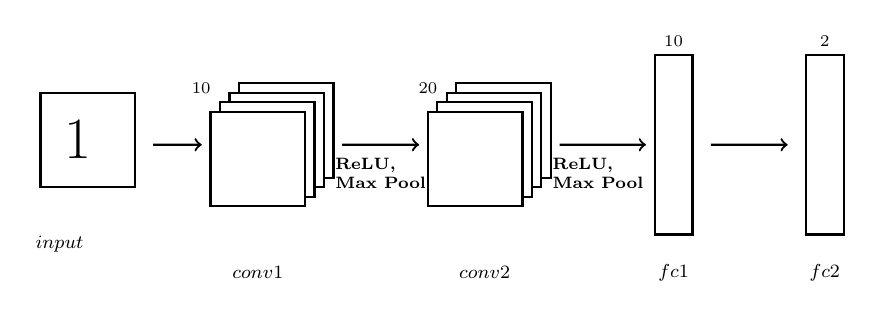
\begin{tikzpicture} [thick,scale=1.2, every node/.style={scale=0.85}]
	
	
	\tikzstyle{arrow} = [line width=1, thick]
	\tikzstyle{arrow1} = [->, line width=1, thick]
	\tikzstyle{arrow2} = [line width=1, draw=red, very thick]
	\tikzstyle{circle1}=[circle,draw=black, thick]
	\tikzstyle{node1}=[text=black, font=\footnotesize \bfseries];
	\tikzstyle{node2}=[text=black, font=\tiny \bfseries];
	\tikzstyle{node3}=[text=black, font=\scriptsize \bfseries];
	\tikzstyle{node4}=[text=black, font=\Huge \bfseries];
	
	\draw [fill=white] (-4.1,0.2) rectangle +(1,1);
	\node [node1] at (-3.9,-0.4){$input$};
	\node [node4] at (-3.7,0.7){$1$};
	
	\node [node1](v15) at (-3,0.65){};
	\node [node1](v16) at (-2.3,0.65){};
	\draw  [arrow1](v15) edge (v16);
	%\node [node3] at (-2.7,0.45){$conv$};
	
	\draw [fill=white] (-2.0,0.3) rectangle +(1,1);
	\draw [fill=white] (-2.1,0.2) rectangle +(1,1);
	\draw [fill=white] (-2.2,0.1) rectangle +(1,1);
	\draw [fill=white] (-2.3,0) rectangle +(1,1);
	\node [node1] at (-1.8,-0.7){$conv1$};
	\node [node3] at (-2.4,1.25){$10$};
	%\node [node2] at (-1.0,-0.1){$\textrm{max}$};
	%\node [node2] at (-1.0,-0.25){$\textrm{pooling}$};
	
	\node [node1](v15) at (-1,0.65){};
	\node [node1](v16) at (0,0.65){};
	\draw  [arrow1](v15) edge (v16);
	\node [node3, align=left] at (-0.5,0.35){ReLU,\\ Max Pool};
	
	\draw [fill=white] (0.3,0.3) rectangle +(1,1);
	\draw [fill=white] (0.2,0.2) rectangle +(1,1);
	\draw [fill=white] (0.1,0.1) rectangle +(1,1);
	\draw [fill=white] (0,0) rectangle +(1,1);
	\node [node3, align=left] at (1.8,0.35){ReLU,\\ Max Pool};
	\node [node1] at (0.6,-0.7){$conv2$};
	\node [node3] at (0,1.25){$20$};
	%\node [node2] at (1.0,-0.25){$\textrm{pooling}$};		
	
	\node [node1](v13) at (1.3,0.65){};
	\node [node1](v14) at (2.4,0.65){};
	\draw  [arrow1](v13) edge (v14);
	%\node [node3] at (1.5,0.45){$dense$};
	
	\draw [fill=white] (2.4,-0.3) rectangle +(0.4,1.9);
	\node [node1] at (2.6,-0.7){$fc1$};
	\node [node3] at (2.6,1.75){$10$};
	
	\node [node1](v11) at (2.9,0.65){};
	\node [node1](v12) at (3.9,0.65){};
	\draw  [arrow1](v11) edge (v12);
	%\node [node3] at (3.0,0.45){$dense$};
	
	\draw [fill=white] (4,-0.3) rectangle +(0.4,1.9);
	\node [node1] at (4.2,-0.7){$fc2$};
	\node [node3] at (4.2,1.75){$2$};
	
	\end{tikzpicture}  
\end{document}
